\newcommand{\dsename}[1]{\textit{#1}}

\vspace{-2pt}
\subsection{UPA Flow and Traversal}
\label{subsec:MAAR}

Novel allocation approaches are needed that broaden the design scope from single application to a set of applications in order to design a unified platform. The enormous design space renders exhaustive search unfeasible, requiring heuristics for sparse sampling. UPA employs an elitist Genetic Algorithm (GA)~\cite{quan2014towards} to support efficient design space traversal.

%\vspace{-4pt}
\begin{figure}[h]
	\centering
	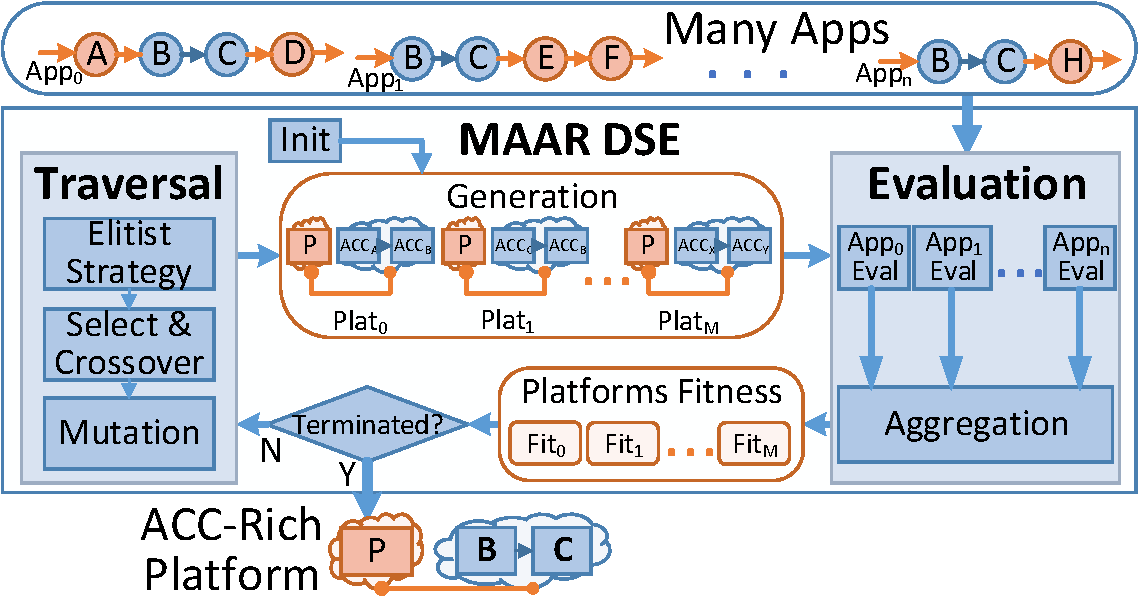
\includegraphics[width=.9\linewidth]{fig/MAARflowDetial.pdf}
	\vspace{-4pt}
	\caption{UPA Flow}
	\label{fig:MAARflowDetial}
\end{figure}

\figref{fig:MAARflowDetial} overviews the UPA flow. The generation's configuration is captured in a set of chromosomes, representing platforms. Each chromosome captures platform allocation of ACCs as a set of genes. After randomly generating an initial generation, the UPA \dsename{Evaluation} analyzes the fitness of each chromosome/platform. In \dsename{Traverse}, the \dsename{Elitist Strategy} tracks global top 10\% platforms (across all generations). It replaces the bottom 10\% each generation with the global top 10\%. From this, \dsename{Selection \& Crossover} selects pairs of promising chromosomes with roulette wheel selection according to their fitness and swaps genes among them. To further speed up exploration, \dsename{Mutation} employs a local search method guided by analytic evaluation to propagate the best neighbor of the design point. The resulting generation is evaluated and the process repeats until the \dsename{Termination} condition (no improvement for 10 iterations) is reached.